\section{Variants of Turing Machines}\label{sec:variantsofturingmachines}

\firstwords{The definition of} a Turing machine that we gave earlier in this lecture is by no means a canonical definition. When we chose to give our machine a deterministic transition function, or a single tape, or a two-way infinite tape, we made those choices simply to fix \emph{some} definition of a Turing machine. Since we are just introducing Turing machines for the first time in this lecture, we decided to go with a relatively easy-to-understand definition: the single, two-way infinite tape allowed us to use our ``two stacks" perspective to motivate the definition, and deterministic transition functions are more straightforward to reason about.

Just like we defined different types of finite automata, nothing is stopping us from modifying our definition of a Turing machine. However, one of the most remarkable results in theoretical computer science is that we can make pretty much \emph{any} modification to our definition of a Turing machine, and it won't affect the recognition power of the model. The Turing machine is, in a sense, the Platonic form of a computer; nearly any variant definition we choose grants us sufficient power to recognize the large classes of decidable and semidecidable languages.

To illustrate, here we will make a number of modifications to our Turing machine definition, and we will then prove that each modified definition is equivalent to our original definition. This will give us a wide array of variant Turing machine models that we can choose from when we're trying to recognize certain languages.

\subsection{Nondeterministic Turing Machines}

The first natural modification we can make to our definition is to take the transition function $\delta$ to be nondeterministic. Just like with our other models of computation, a nondeterministic transition function for a Turing machine will map a pair of state and tape symbol to the power set of tuples of state, tape symbol, and input head movement.

\begin{definition}[Nondeterministic Turing machine]\label{def:nondeterministicTM}
\sloppy A nondeterministic Turing machine is a tuple $(Q, \Sigma, \Gamma, \delta, q_{0}, \allowbreak q_{\text{accept}}, q_{\text{reject}})$, where everything is defined as in Definition~\ref{def:TM} except for the transition function, which is
\begin{equation*}
\delta: \left( Q \setminus \{q_{\text{accept}}, q_{\text{reject}}\} \right) \times \Gamma \to \mathcal{P}\left( Q \times \Gamma \times \{L, R\} \right).
\end{equation*}
\end{definition}

We saw that deterministic and nondeterministic finite automata are equivalent in terms of recognition power, while nondeterministic pushdown automata are able to recognize more languages than deterministic pushdown automata. With Turing machines, we return to equivalence: adding nondeterminism to a Turing machine does not give it more recognition power.

\begin{theorem}\label{thm:NTMDTMequivalent}
Given a nondeterministic Turing machine $\mathcal{M}$, we can construct a deterministic Turing machine $\mathcal{M}'$ such that $L(\mathcal{M}') = L(\mathcal{M})$.

\begin{proof}
Let $\mathcal{M} = (Q, \Sigma, \Gamma, \delta, q_{0}, q_{\text{accept}}, q_{\text{reject}})$ be a nondeterministic Turing machine. We will construct a deterministic Turing machine $\mathcal{M}'$ that uses three tapes to simulate the nondeterministic computation of $\mathcal{M}$.
\begin{itemize}
\item The first tape will be the \emph{input tape}, and it will contain the input word given to $\mathcal{M}$. The contents of the input tape will not be changed during the computation.
\item The second tape will be the \emph{simulation tape}, and it will simulate the contents of $\mathcal{M}$'s tape as $\mathcal{M}$ performs its nondeterministic computation.
\item The third tape will be the \emph{address tape}, and it will keep track of where we are in the nondeterministic computation tree of $\mathcal{M}$.
\end{itemize}
Before we proceed, let's consider how we can represent the nondeterministic computation tree of $\mathcal{M}$ on a linear form of storage like a tape. If we take $b$ to denote the maximum number of branches in the tree (that is, the maximum number of nondeterministic transitions $\mathcal{M}$ can follow at any given point in its computation), then we can assign a unique address to each vertex of the tree over the alphabet $\Sigma_{b} = \{1, 2, \dots, b\}$. The address is determined by tracing the branches we must follow in order to get from the root to that vertex; for example, the vertex with address $123$ can be reached by starting at the root of the tree and taking the first branch, followed by the second branch, followed by the third branch. As a consequence of this convention, the root of the tree receives the address $\epsilon$.

\begin{center}
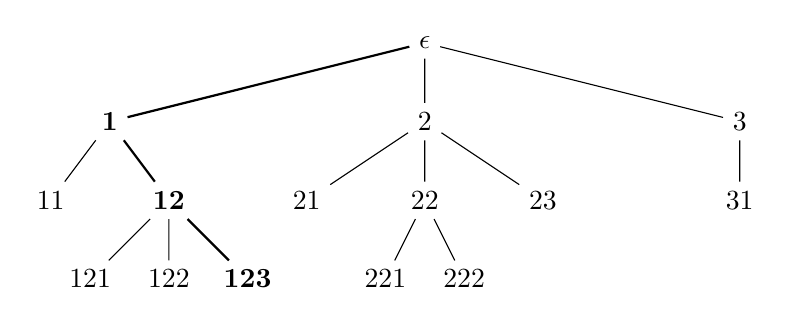
\begin{tikzpicture}[emph/.style={edge from parent/.style={draw,\maincolour,thick}},norm/.style={edge from parent/.style={draw,black,thin}}]
\node[\maincolour] {$\bm\epsilon$} [level 1/.style={sibling distance=4cm}, level 2/.style={sibling distance=1.5cm}, level 3/.style={sibling distance=1cm}, level distance=1cm]
	child[emph] {node[\maincolour] {\textbf{1}}
		child[norm] {node {11}}
		child[emph] {node[\maincolour] {\textbf{12}}
			child[norm] {node {121}}
			child[norm] {node {122}}
			child[emph] {node[\maincolour] {\textbf{123}}}
		}
	} 
	child {node {2}
		child {node {21}}
		child {node {22}
			child {node {221}}
			child {node {222}}
		}
		child {node {23}}
	}
	child {node {3}
		child {node {31}}
	};
\end{tikzpicture}
\end{center}

The address tape, then, contains symbols from the alphabet $\Sigma_{b}$. Each symbol on the address tape will tell $\mathcal{M}'$ which branch of the nondeterministic computation tree it must follow in its next computation step. Note that the contents of the address tape do not necessarily need to correspond to a vertex of the tree; if the address tape contains an invalid address, then $\mathcal{M}'$ simply aborts its attempted simulation of that branch.

Having defined the three tapes, we can describe how $\mathcal{M}'$ simulates the computation of $\mathcal{M}$:
\begin{enumerate}
\item Initialize the tapes in the following way: 
	\begin{enumerate}
	\item Copy the contents of the input tape to the simulation tape; that is, write the input word $w$ given to $\mathcal{M}$ to the simulation tape.
	\item Leave the address tape empty.
	\end{enumerate}
\item Use the simulation tape to perform the following steps:
	\begin{enumerate}
	\item For each computation step of $\mathcal{M}$, read the next symbol of the address tape to determine which branch of the nondeterministic computation tree to follow.
	\item If there are no more symbols remaining on the address tape, or if the address tape contains an invalid address, or if $\mathcal{M}$ enters a rejecting configuration, then abort the attempted simulation of this branch and go to step 3.
	\item If $\mathcal{M}$ enters an accepting configuration, then accept $w$.
	\end{enumerate}
\item Write to the address tape the sequence of symbols over $\Sigma_{b}$ that comes next in lexicographic order and go to step 2. \qedhere
\end{enumerate}
\end{proof}
\end{theorem}

Since every deterministic Turing machine is a nondeterministic Turing machine that doesn't use nondeterminism during its computation, we immediately obtain the other direction of the relationship between these models. Therefore, we can conclude that deterministic and nondeterministic Turing machines are equivalent.

\subsection{Multitape Turing Machines}

In the proof of Theorem~\ref{thm:NTMDTMequivalent}, we saw that we could simulate the computation of a nondeterministic Turing machine using a deterministic Turing machine with multiple tapes. It's natural to wonder whether including additional tapes gave us some kind of advantage in this simulation process---after all, giving our computational model two stacks instead of one stack led us to the idea of a Turing machine---but as it turns out, we can perform exactly the same computations using only a single tape.

First, let's define our \emph{multitape Turing machine} model. Again, we only need to modify the transition function: instead of mapping a pair of state and \emph{one} tape symbol to a tuple of state, \emph{one} tape symbol, and \emph{one} input head movement, we will transition on $k$ tape symbols and $k$ input head movements, where $k$ denotes the number of tapes used by the machine.

\begin{definition}[$k$-tape Turing machine]\label{def:multitapeTM}
A $k$-tape Turing machine is a tuple $(Q, \Sigma, \Gamma, \delta, q_{0}, q_{\text{accept}}, q_{\text{reject}})$, where everything is defined as in Definition~\ref{def:TM} except for the transition function, which is
\begin{equation*}
\delta: \left( Q \setminus \{q_{\text{accept}}, q_{\text{reject}}\} \right) \times \Gamma^{k} \to Q \times \Gamma^{k} \times \{L, R\}^{k}.
\end{equation*}
\end{definition}

The idea allowing us to establish one direction of the equivalence between multitape and single-tape Turing machines is that we can simulate having many tapes $T_{i}$ by storing all of the contents on a single tape $T$ and separating ``tape $i$" from the other ``tapes" using a special symbol. Since our single tape has only one input head, we will also simulate the position of each input head on ``tape $i$" using a special marker on the corresponding tape symbol to act as a virtual input head.

\begin{figure}
\centering
\begin{tikzpicture}[%
	tape1/.style={rectangle split, rectangle split horizontal, rectangle split parts=#1, rectangle split part align=base, draw, anchor=center, rectangle split part fill={white,white,white,white,white,\fourthcolour,white,white,white,white}},%
	tape2/.style={rectangle split, rectangle split horizontal, rectangle split parts=#1, rectangle split part align=base, draw, anchor=center, rectangle split part fill={white,white,white,white,\fourthcolour,white,white,white,white,white}},%
	tape3/.style={rectangle split, rectangle split horizontal, rectangle split parts=#1, rectangle split part align=base, draw, anchor=center, rectangle split part fill={white,\fourthcolour,white,white,white,white,white,white,white,white}}%
	]
\node[tape1=10] (tp1) {
\nodepart{one}$\cdots$
\nodepart{two}$\blankspace$
\nodepart{three}\texttt{a}
\nodepart{four}\texttt{b}
\nodepart{five}\texttt{b}
\nodepart{six}\color{\maincolour}\texttt{a}
\nodepart{seven}\texttt{a}
\nodepart{eight}\texttt{b}
\nodepart{nine}$\blankspace$
\nodepart{ten}$\cdots$
};
\node[tape2=10, below=0em of tp1] (tp2) {
\nodepart{one}$\cdots$
\nodepart{two}$\blankspace$
\nodepart{three}$\blankspace$
\nodepart{four}\texttt{0}
\nodepart{five}\color{\maincolour}\texttt{1}
\nodepart{six}\texttt{1}
\nodepart{seven}\texttt{0}
\nodepart{eight}$\blankspace$
\nodepart{nine}$\blankspace$
\nodepart{ten}$\cdots$
};
\node[tape3=10, below=0em of tp2] (tp3) {
\nodepart{one}$\cdots$
\nodepart{two}\color{\maincolour}\texttt{c}
\nodepart{three}\texttt{c}
\nodepart{four}\texttt{d}
\nodepart{five}\texttt{d}
\nodepart{six}\texttt{c}
\nodepart{seven}\texttt{c}
\nodepart{eight}\texttt{d}
\nodepart{nine}\texttt{d}
\nodepart{ten}$\cdots$
};
\end{tikzpicture}

\smallskip
$\Downarrow$
\medskip

\begin{tikzpicture}[tape/.style={fill=white, rectangle split, rectangle split horizontal, rectangle split parts=#1, rectangle split part align=base, draw, anchor=center}]
\node[tape=17] (tp) {
\nodepart{one}$\cdots$
\nodepart{two}$\blankspace$
\nodepart{three}\texttt{\#}
\nodepart{four}\texttt{a}
\nodepart{five}\texttt{b}
\nodepart{six}\texttt{b}
\nodepart{seven}$\bigdot{\texttt{a}}$
\nodepart{eight}\texttt{a}
\nodepart{nine}\texttt{b}
\nodepart{ten}\texttt{\#}
\nodepart{eleven}\texttt{0}
\nodepart{twelve}$\bigdot{\texttt{1}}$
\nodepart{thirteen}\texttt{1}
\nodepart{fourteen}\texttt{0}
\nodepart{fifteen}\texttt{\#}
\nodepart{sixteen}$\bigdot{\texttt{c}}$
\nodepart{seventeen}$\cdots$
};
\end{tikzpicture}
\caption{Simulating the computation of a $k$-tape Turing machine (top) with a single-tape Turing machine (bottom). The positions of the $k$ physical input heads are indicated by highlighted cells, while the corresponding $k$ virtual input heads are indicated by dots}
\label{fig:TMktapeto1tape}
\end{figure}

\begin{theorem}\label{thm:ktapeequivalent}
Given a $k$-tape Turing machine $\mathcal{M}$, we can construct a single-tape Turing machine $\mathcal{M}'$ such that $L(\mathcal{M}') = L(\mathcal{M})$.

\begin{proof}
Suppose the given Turing machine $\mathcal{M}$ has $k$ tapes, and the tape alphabet is denoted by $\Gamma$. Our single-tape Turing machine $\mathcal{M}'$ will simulate $\mathcal{M}$'s computation on an input word $w = w_{1} \dots w_{n}$ in the following way: 
\begin{enumerate}
\item Take the tape alphabet of $\mathcal{M}'$ to be $\Gamma' = \Gamma \cup \bigdot{\Gamma} \cup \{\texttt{\#}\}$, where $\bigdot{\Gamma}$ consists of all alphabet symbols of $\Gamma$ augmented with a dot and \texttt{\#} is a special boundary marker.
\item Write the boundary marker \texttt{\#} and the symbols of $w$ to the tape of $\mathcal{M}'$, including the dotted symbol $\bigdot{w_{1}}$. Then, write $k+1$ copies of \texttt{\#} each separated by a dotted blank space.
\begin{center}
\begin{tikzpicture}[tape/.style={fill=white, rectangle split, rectangle split horizontal, rectangle split parts=#1, rectangle split part align=base, draw, anchor=center}]
\node[tape=12] (tp) {
\nodepart{one}$\cdots$
\nodepart{two}$\blankspace$
\nodepart{three}\texttt{\#}
\nodepart{four}$\bigdot{w_{1}}$
\nodepart{five}$\dots$
\nodepart{six}$w_{n}$
\nodepart{seven}\texttt{\#}
\nodepart{eight}$\bigdot{\blankspace}$
\nodepart{nine}\texttt{\#}
\nodepart{ten}$\bigdot{\blankspace}$
\nodepart{eleven}\texttt{\#}
\nodepart{twelve}$\cdots$
};
\end{tikzpicture}
\end{center}
\item For each step of the computation, $\mathcal{M}'$ scans its entire tape from the first occurrence of \texttt{\#} to the $(k+1)$st occurrence of \texttt{\#} to read the symbols on all $k$ tapes of $\mathcal{M}$. Then, $\mathcal{M}'$ makes a second pass along its tape to update any symbols that were changed by the transition function of $\mathcal{M}$. This update includes changing occurrences of dotted symbols in accordance with the changed positions of each virtual input head.

If any of the virtual input heads of $\mathcal{M}'$ move onto an occurrence of \texttt{\#}, then $\mathcal{M}$ must have moved the corresponding input head of that tape onto a blank space. In this case, $\mathcal{M}'$ writes a blank space to this cell of its tape and shifts the symbols of all subsequent cells rightward by one position. \qedhere
\end{enumerate}
\end{proof}
\end{theorem}

The process of condensing the contents of all $k$ tapes onto a single tape is illustrated in Figure~\ref{fig:TMktapeto1tape}. Naturally, a $k$-tape Turing machine can simulate the computation of a single-tape Turing machine by using only one of its $k$ tapes. This again gives us the other direction of the relationship between the models, and again establishes the equivalence of the models.

\subsection{One-Way Infinite Tape Turing Machines}

In our definition of a Turing machine, we assumed that the tape used by the machine is \emph{two-way infinite}; that is, there is an infinite number of cells to the left and to the right of the input head, and the input head can therefore move to an infinite number of positions of the tape in either direction.

We didn't have to define our storage in this way, though. We could have alternatively defined the tape to act more like the stack of a pushdown automaton: just like the stack has a fixed bottom boundary forcing us to push symbols only above that boundary, the tape could have a fixed left boundary forcing us to write symbols only to the right of that boundary. We call such a tape \emph{one-way infinite}, since at any position along the tape, the input head has a finite number of cells to its left and an infinite number of cells to its right.

Because of the way the computation of the Turing machine begins, the initial position of the input head of a Turing machine with a one-way infinite tape will be on the first symbol of the input word, and the left boundary of the tape will be to the input head's immediate left. In this cell, the input head cannot make a leftward move; if the transition function tells the input head to move left, then the input head will simply remain in the same cell by making a rightward move immediately followed by a leftward move.

\begin{remark}
Some authors alternatively assert that, if the input head of a one-way infinite tape Turing machine moves beyond the left boundary of the tape, then the machine ``crashes" and the computation cannot continue.
\end{remark}

If we want to simulate the computation of a one-way infinite tape Turing machine using a two-way infinite tape Turing machine, then the required conversion seems straightforward: we just need to write a special symbol to one cell of the two-way infinite tape to act as the left boundary, and modify the transition function to handle the case where the input head moves onto this left boundary marker.

\begin{figure}
\centering
\begin{tikzpicture}[tape/.style={fill=white, rectangle split, rectangle split horizontal, rectangle split parts=#1, rectangle split part align=base, draw, anchor=center}]
\node[tape=6] (tp) {
\nodepart{one}\texttt{a}
\nodepart{two}\texttt{b}
\nodepart{three}\texttt{b}
\nodepart{four}\texttt{a}
\nodepart{five}$\blankspace$
\nodepart{six}$\cdots$
};
\end{tikzpicture}

\smallskip
$\Downarrow$
\medskip

\begin{tikzpicture}[tape/.style={fill=white, rectangle split, rectangle split horizontal, rectangle split parts=#1, rectangle split part align=base, draw, anchor=center}]
\node[tape=10] (tp) {
\nodepart{one}$\cdots$
\nodepart{two}$\blankspace$
\nodepart{three}$\blankspace$
\nodepart{four}$\vdash$
\nodepart{five}\texttt{a}
\nodepart{six}\texttt{b}
\nodepart{seven}\texttt{b}
\nodepart{eight}\texttt{a}
\nodepart{nine}$\blankspace$
\nodepart{ten}$\cdots$
};
\end{tikzpicture}
\caption{Simulating the computation of a one-way infinite tape Turing machine (top) with a two-way infinite tape Turing machine (bottom)}
\label{fig:TMonewaytotwoway}
\end{figure}

\begin{theorem}\label{thm:onewayequivalent}
Given a one-way infinite tape Turing machine $\mathcal{M}$, we can construct a two-way infinite tape Turing machine $\mathcal{M}'$ such that $L(\mathcal{M}') = L(\mathcal{M})$.

\begin{proof}
Suppose the given one-way infinite tape Turing machine $\mathcal{M}$ receives as input a word $w = w_{1} \dots w_{n}$ and has a tape alphabet $\Gamma$. Our two-way infinite tape Turing machine $\mathcal{M}'$ will simulate $\mathcal{M}$'s computation on $w$ in the following way:
\begin{enumerate}
\item Take the tape alphabet of $\mathcal{M}'$ to be $\Gamma' = \Gamma \cup \{\vdash\}$, where $\vdash$ is a special left boundary marker.
\item Write the symbols of $w$ to the tape of $\mathcal{M}'$, and write the left boundary marker $\vdash$ in the cell to the immediate left of the cell containing $w_{1}$.
\item Take the transition function of $\mathcal{M}'$ to be $\delta' = \delta$ and, for each state $q \in Q$, add a new transition $\delta'(q, \vdash) = (q, \vdash, R)$ to the transition function of $\mathcal{M}'$.
\item Create new states $q'_{\text{accept}}$ and $q'_{\text{a}}$, and add new transitions to the transition function of $\mathcal{M}'$ as follows:
	\begin{itemize}
	\item $\delta'(q_{\text{accept}}, \vdash) = (q'_{\text{accept}}, \vdash, R)$;
	\item $\delta'(q_{\text{accept}}, c) = (q'_{\text{a}}, c, R)$ for all $c \in \Gamma' \setminus \{\vdash\}$; and
	\item $\delta'(q'_{\text{a}}, d) = (q'_{\text{accept}}, d, L)$ for all $d \in \Gamma' \setminus \{\vdash\}$.
	\end{itemize}
Also, create new states $q'_{\text{reject}}$ and $q'_{\text{r}}$, and add similar transitions on these states. Take the accepting and rejecting states of $\mathcal{M}'$ to be $q'_{\text{accept}}$ and $q'_{\text{reject}}$, respectively. \qedhere
\end{enumerate}
\end{proof}
\end{theorem}

The construction described in Theorem~\ref{thm:onewayequivalent} is illustrated in Figure~\ref{fig:TMonewaytotwoway}.

\begin{figure}
\centering
\begin{tikzpicture}[tape/.style={fill=white, rectangle split, rectangle split horizontal, rectangle split parts=#1, rectangle split part align=base, draw, anchor=center}]
\node[tape=10] (tp) {
\nodepart{one}$\cdots$
\nodepart{two}$\blankspace$
\nodepart{three}$\blankspace$
\nodepart{four}\texttt{a}
\nodepart{five}\texttt{b}
\nodepart{six}\texttt{b}
\nodepart{seven}\texttt{a}
\nodepart{eight}\texttt{a}
\nodepart{nine}\texttt{b}
\nodepart{ten}$\cdots$
};
\end{tikzpicture}

\smallskip
$\Downarrow$
\medskip

\begin{tikzpicture}[tape/.style={fill=white, rectangle split, rectangle split horizontal, rectangle split parts=#1, rectangle split part align=base, draw, anchor=center}]
\node[tape=8] (tp1) {
\nodepart{one}\texttt{a}
\nodepart{two}\texttt{b}
\nodepart{three}\texttt{b}
\nodepart{four}\texttt{a}
\nodepart{five}\texttt{a}
\nodepart{six}\texttt{b}
\nodepart{seven}$\blankspace$
\nodepart{eight}$\cdots$
};
\node[tape=8, below=0em of tp1] (tp2) {
\nodepart{one}$\blankspace$
\nodepart{two}$\blankspace$
\nodepart{three}$\blankspace$
\nodepart{four}$\blankspace$
\nodepart{five}$\blankspace$
\nodepart{six}$\blankspace$
\nodepart{seven}$\blankspace$
\nodepart{eight}$\cdots$
};
\path[<->, >=latex, color=\maincolour] ($(tp1.west)+(-0.2,0)$) edge[thick, bend right=90, min distance=1.25em] ($(tp2.west)+(-0.2,0)$);
\end{tikzpicture}
\caption{Simulating the computation of a two-way infinite tape Turing machine (top) with a one-way infinite tape Turing machine (bottom)}
\label{fig:TMtwowaytooneway}
\end{figure}

To obtain the other direction of the equivalence---that is, to simulate the computation of a two-way infinite tape Turing machine with a one-way infinite tape Turing machine---we can use our previous result establishing the equivalence of single-tape and multitape Turing machines.

While we won't go through the full proof here, the idea is to split the two-way infinite tape into a pair of one-way infinite tapes, where the ``split point" occurs between the first symbol of the input word and the infinite blank spaces to the left of the input word. This action produces two one-way infinite tapes: one containing the input word, and one containing only blank spaces. Then, we modify the transition function of the one-way infinite tape Turing machine to operate on either the first or second tape, switching between the tapes each time the input head of the two-way infinite tape Turing machine crosses the ``split point" on its tape.

Splitting the two-way infinite tape into a pair of one-way infinite tapes gives us the setup depicted in Figure~\ref{fig:TMtwowaytooneway}, where the two-way infinite tape is, in effect, folded in half. Ultimately, this construction completes the proof and establishes the equivalence between one-way and two-way infinite tape Turing machines.

%\subsection{Turing Machines with No-Ops}